% Chapter 1
% Chapter Template
\chapter{Introduction} % Main chapter title
\label{Chapter1} % Change X to a consecutive number; for referencing this chapter elsewhere, use \ref{ChapterX}

%\lhead{Chapter 1. \emph{Introduction}} % Change X to a consecutive number; this is for the header on each page - perhaps a shortened title
\renewcommand{\chaptermark}[1]{\markboth{#1}{}}
\renewcommand{\sectionmark}[1]{\markright{#1}}
\fancyhead[RE]{\small\leftmark}
% Section in the left on even pages}
\fancyhead[LO]{\small\rightmark}%Section in the left on odd pages

%\section{A section goes here}

Evolution has yielded an immense diversity of microbial functions. Today, many of those functions remain uncharacterized and exploring the unknown taxa and functions of the world\textquotesingle s microbiomes should be a \quotes{central priority for biologists} \citep{Bernard_2018}. Even after a century of functional characterization of the model organism \textit{Saccharomyces cerevisiae}, greater than 30\% of its protein coding sequences do not have a clear function \citep{Ellens_2017}. To shed light on the unknown functions of the microbial world, an important first step is to categorize and quantify how much is already known and how much is not known. With modern sequencing technologies and large scale sampling projects, this is now possible.\\

The emerging fields of metagenomics and shotgun sequencing have allowed for the description of the total genetic content in environmental samples. Rather than amplifying specific target DNA sequences (i.e. amplicon studies), metagenomics has the potential to simultaneously unveil both function and taxonomy of the microorganisms present in a sample. This allows for the comparison and quantification of differences in microbial physiological traits between sites. With the onset of next generation sequencing (NGS), cost per sequence has dramatically decreased down to 1 cent per megabase (https://www.genome.gov/sequencingcostsdata/, accessed 12.03.2018). Owing to this, large scale metagenomics sampling projects such as Global Ocean Sampling (GOS) \citep{Rusch_2007}, TARA Oceans \citep{Sunagawa_2015}, and Ocean Sampling Day (OSD) \citep{Kopf_2015} have sampled the world\textquotesingle s oceans and added terabytes of novel sequence data to databases. \\

GOS was the first attempt to create a snapshot of ocean genetic diversity with some of the largest sampling transects and collections of metadata ever accomplished \citep{Rusch_2007}. Its dataset generated 6.12 million open reading frames (ORFs) from its Sanger sequencing long reads \citep{Yooseph_2007}. Additionally, the GOS dataset lead to fascinating insights into marine microbial ecology, including the elucidation of the ocean\textquotesingle s dominant microbial genomes (i.e. \textit{Prochlorococcus} and SAR-11) and uncovering more microbial diversity in the ocean than previously thought \citep{Nealson_2007, Venter_2004, Rusch_2007, Yooseph_2007}.\\

Inspired by the GOS dataset, The TARA Oceans Expedition went a step further, not only increasing the breadth of sampling, but adding a systematic exploration of the sunlit ocean with the addition of more filter fractions and depths, and unprecedented sequencing depth. The first analysis of the prokaryotic fraction of the TARA dataset yielded a 40 million non-redundant reference gene catalogue \citep{Sunagawa_2015}. Later, a metatranscriptome analysis of the eukaryotic fraction added a separate 116 million non-redundant reference gene catalogue \citep{Carradec_2018}. Investigation into the prokaryotic dataset uncovered temperature as the main driver of microbial function and diversity, and revealed that the core functionality of the ocean microbiome compared to the human microbiome is 73\% similar \citep{Sunagawa_2015}.\\

\textbf{From data to knowledge}\\

Microbial knowledge discovery from GOS and TARA would not have been possible without the ability for predicted genes (i.e. open reading frames - ORFs) to be annotated. With annotated ORFs, overall community functional fingerprints can be compared between samples. Analysis of the TARA ocean data revealed that upon aggregation of functions within metagenomes, there is functional redundancy throughout the world\textquotesingle s ocean \citep{Louca_2016}. Yet, due to the sheer number of ORFs generated from these datasets, in the recent years, a variety of tools have been developed to efficiently compare and annotate environmental sequences with characterized sequences in databases. Algorithmic improvements to the original BLAST program \citep{Altschul_1990}, like DIAMOND \citep{Buchfink_2014} or MMSEQS2 \citep{Steinegger_2017} have allowed for local alignments of query sequences against a target sequence database in a high-throughput manner. However, sequence similarity based annotation methods have limitations if the scientific question at hand is detecting remote homologies or accurately assigning function. In fact, sequence similarity does not inherently imply homology or function, but is merely a metric to describe nucleotide resemblance \citep{States_1991}. To detect functional similarity and/or investigate evolutionary based questions of proteins (e.g. homologues, paralogues, and conserved domains), profile based tools should additionally be used.\\

A common way to create protein profiles is by calculating Hidden Markov Models (HMM) from multiple sequence alignments (MSAs) of protein families. Pfam \citep{Finn_2015} is an example of a profile database that manually curates protein families of highly conserved functional regions within proteins called domains. Other examples of protein family profile databases are Clusters of Orthologous Genes (COG) \citep{Tatusov_2000}, SFams \citep{Sharpton_2012}, and eggNOG \citep{Huerta_Cepas_2015}. Protein profile databases differ in their curation methodology, but manual curation of protein families is the best way to ensure high quality. This is because an expert can add biological context to a protein family\textquotesingle s MSA and identify the spurious members. Unfortunately, due to the size of nucleotide databases and large metagenome projects, the amount of sequences now far outweighs the time constraints of manual definition and curation of protein families.\\

To handle this amount of data, unsupervised clustering algorithms are being used to define an initial set of related proteins. These algorithms follow two main approaches, graph based and sequence similarity based \citep{Pavlopoulos_2017}. Graph based clustering algorithms start by performing an all-versus-all alignment using tools like DIAMOND or BLAST. Next, they create a sequence similarity network (SSN) using on the criterion of the alignment (e.g. e-value) as edges, then perform a clustering of the SSN to extract components as protein families (MCL is an example of a popular method \citep{Enright_2002}). On the other hand, tools that are based on sequence similarity grouping use k-mer frequencies (MMSEQS2 \citep{Steinegger_2017}, CD-HIT \citep{Li_2006}, UCLUST \citep{Edgar_2010}). One characteristic of the latter methods is their increased speed. With this, they are well suited to be applied to the massive metagenomic data sets.\\

In fact, one way to explore protein family diversity of environmental metagenomic ORFs is to cluster them with already recovered ORFs sequences in databases. This can lead to previously characterized protein families being expanded, shrunk, or the creation of novel families. GOS took this approach and yielded 1,700 clusters (grouped sequences after clustering) with no detectable homology or function \citep{Yooseph_2007}. Although new families may emerge when including new sequences, some may have a known function, but a vast majority will remain unknown.\\

\textbf{De-bunking the unknown}\\

There have been different strategies to expand annotations to unknown protein families including protein structure/sequence similarity analysis and domain co-occurrence networks. \cite{Jaroszewski_2009} structurally characterized 250 PFAM domains of unknown function (DUFs) using structural genomics. After comparing DUFs to known proteins on a structural level, it was determined that most of the DUFs were distant variants and not completely novel. \cite{Mudgal_2015} expanded upon this work with increased sensitivity and higher quality structural databases which lead to 20\% of DUFs being annotated as distantly related domains. Both studies discuss that the protein universe may soon be saturated from a structural perspective and most \quotes{novel} sequences are due to protein diversification from environmental niche selection. Based on the assumption that DUFs are products of niche adaptation, \cite{Buttigieg_2013} postulated that DUFs may co-occur with domains of known function between metagenomic samples. To explore this, they calculated the co-occurrence of DUFs with characterized domains in the GOS dataset and used correlation and network exploration to infer function, i.e. \quotes{guilty by association} method.\\

Even after deploying different strategies to annotate functions to new protein families, some families remain unknown. It is then an important step to confirm clusters that do not have detectable homology or function, are indeed novel and legitimate biological entities. This is a unique challenge in metagenomic data due to short reads, insufficient sequencing depth \citep{Parks_2011, Barrientos_Somarribas_2018}. Moreover, gene prediction algorithms have limitations and can yield inaccurate ORFs predictions leading to spurious proteins, which can lead to spurious protein families. Dedicated databases have been curated to detect and remove spurious proteins (e.g. AntiFAM \citep{Eberhardt_2012}). Additionally, specific tools like Spurio \citep{H_ps_2018} have been designed to score query ORFs on their likelihood of being spurious.\\

Another strategy to confirm protein family novelty is to determine if the members of the cluster are under positive or negative selective pressure by calculating non-synonymous to synonymous substitutions (Ka/Ks) \citep{Yooseph_2007, Barrientos_Somarribas_2018}. If ORFs have a Ka/Ks value close to 1, there is a strong indication for no selective pressure, thus a predicted ORF may not be a real coding sequence \citep{Nekrutenko_2001}. One issue with this validation strategy is, it assumes that all proteins in a metagenomic sample are under the same environmental pressures. When filtering out novel clusters with the criteria of Ka/Ks being closed to one, an assumption is made that all proteins are under purifying selection.

\textbf{Categorizing the unknown}\\

Even after various strategies to expand annotations and debunk unknown clusters, numerous protein families still indeed remain with unknown functions. The concept of \quotes{unknowns} in microbiology is a recognized problem that has implications for both fundamental and applied biological research. The term \quotes{biological dark matter} was first used by \cite{Marcy_2007} to describe the uncultured majority of microbes that could only be indirectly detected via environmental sequencing methods. Later, the term would also be used to refer to protein families with no detectable homology to characterized proteins from sequenced genomes \citep{Ellens_2017, Perdig_o_2017, Roux_2015, Fischer_1999}.\\

When categorizing and defining the unknown, it is important to quantify in reality how much is already known. \cite{Perdig_o_2017} approached the unknowns from a structural perspective by making the \quotes{Dark Proteome Database}. Protein sequences are ranked on a scale of \quotes{darkness} based on how confidently parts or the whole sequence can have of an inferred 3D structure. This is done by calculating MSAs to protein structural databases. Wyman et al., 2017 categorized SFams (clusters created via a graph-based approach from sequences of genomes) as FUnkFams (protein families of unknown function) if the clusters could not be annotated by the Pfam or the NCBI Conserved Domain database.\\

For this thesis, I used the clusters of ORFs produced from the work of Vanni et. al. (in prep.)(\url{https://orcid.org/0000-e2-1124-1147}). This workflow builds upon the motivations of the methods mentioned above but focuses on ORF cluster validation and deeper categorization of the unknown. Vanni et. al. used MMSEQS2 to cluster the 322,248,552 ORFs from The Human Microbiome Project (HMP), TARA Oceans \citep{Sunagawa_2015}, Ocean Sampling Day (OSD) \citep{Kopf_2015}, Global Ocean Sampling Expedition (GOS) \citep{Yooseph_2007}, and Malaspina \citep{Duarte_2015}. This dataset yielded 32,465,074 clusters that were then validated downstream. In parallel to clustering, the ORF dataset received Pfam annotations which were used to assist in cluster validation and unknown categorization.\\

Cluster validation is a critical step to protein clustering because unsupervised clustering algorithms can include non-biologically relevant ORFs into clusters due to incomplete or spurious ORFs gene duplications, and genome rearrangements. Vanni et. al. validated clusters for compositional and functional homogeneity. At the end of the validation steps, 2,953,903 clusters were successfully passed on to be categorized in terms of their level of unknown.\\

The goal of the categorization was to quantify the amount of novel versus characterized clusters based on the ability to annotate their function. For this purpose, the ORF cluster space was classified in the following categories:\\

\textbf{Knowns with PFAM (Knowns)}\\
ORF clusters that have been annotated with a PFAM domains of known function.\\
\textbf{Knowns without PFAMs (Kwp)}\\
ORF clusters that have a known function but do not contain PFAM annotations.\\
\textbf{Genomic Unknowns (GUs)}\\
ORF clusters that have an unknown function (e.g. DUF, hypothetical protein) but are found in sequenced or draft-genomes.\\
\textbf{Environmental Unknowns (EUs)}\\
ORF clusters with an unknown function and are not found in sequenced or draft-genomes.\\

%A figure

\begin{figure}[h!]
	\centering
	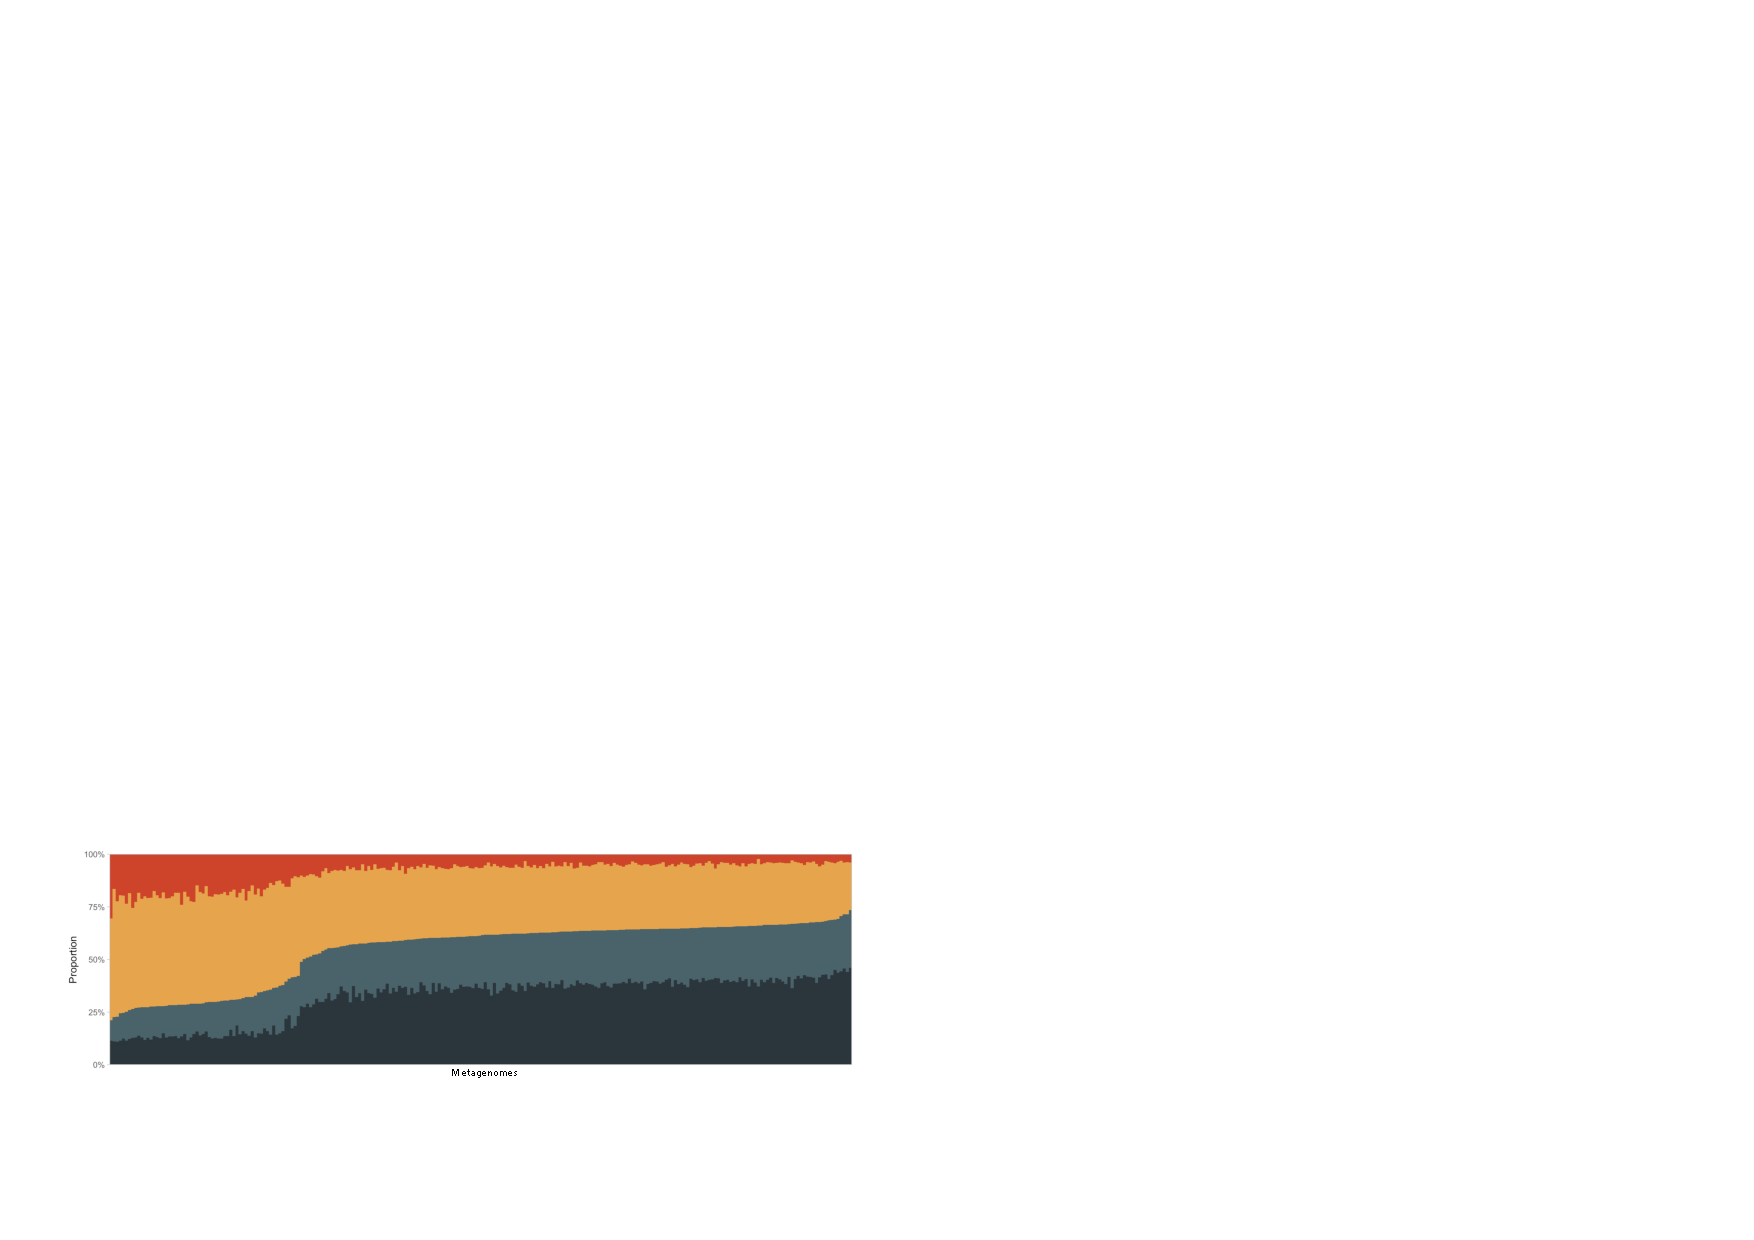
\includegraphics[width=1.0\textwidth] {fig_1.pdf}
	\caption[Proportions of Vanni et. al. cluster categories in the TARA Ocean metagenomes]{\textbf{Proportions of Vanni et. al. cluster categories in the TARA Ocean metagenomes.} The X axis denotes each of the TARA metagenomes while the Y axis is the relative proportion of the different Vanni et. al. cluster categories. Some of the metagenomes have greater than 70\% Unknowns. (Red = EUs; Yellow = GUs; Blue=Knowns; Black = Kwp)}\label{fig1}
\end{figure}

In 16S ribosomal DNA (rDNA) amplicon studies, amplified sequences are clustered together to form operational taxonomic units (OTU). This is advantageous because it reduces the data set for downstream computations and allows for annotation of the cluster representative with taxonomy. If each individual amplicon was treated as an OTU, alpha and beta diversity measurement computations would be very expensive thus making low resolution hypotheses about diversity difficult to make. A similar idea was applied by Vanni et. al. to their dataset to aggregate clusters into larger components due to the Known clusters exhibiting domain architecture redundancy. This may have been caused by the limitations of the clustering method used (based on sequence similarity) to detect distant homologies and the threshold selected (30\% of similarity), resulting in multiple clusters with the same domain architecture. \\

In total, there were 9,687 clusters with more than one PFAM annotation and 18,368 PFAM annotation combinations in the final clusters. To address this, they used the consensus sequence of the Knowns to create a sequence similarity network (SSN) and extracted components.\\

The term \quotes{components} will now be used for the rest of this thesis to describe aggregated clusters occurring in the TARA ocean dataset.\\

\textbf{Aim of this thesis}\\

The cluster components are ideal to address the main objective of this thesis - the exploration of the ecological significance and functional biogeography of the unknown functional diversity in the world\textquotesingle s oceans.\\

To echo back to the 16S rDNA amplicon analogy discussed previously, OTUs that do not receive a taxonomical annotation can still be included in ecological analyses. In this thesis, I use this philosophy but with unannotated ORF components. In the TARA Ocean data set, some samples have greater than 70\% of the metagenome categorized as unknown (Fig.~\ref{fig1}). Until now a large proportion of this functionally uncharacterized fraction has not been used for the study of the prokaryotic fraction \citep{Roux_2015}. In this thesis, it is demonstrate that including the whole metagenomic sample (Knowns and Unknowns) adds more variance to sample site ordinations. Also, it is shown that utilizing the unknowns in functional biogeography can lead to new insights into genetic differences between sites in different ocean regions. Finally, it is shown that there is a potential group of EU proteins that are ubiquitous throughout the ocean. To increase the evidence that the detected ubiquitous EUs are indeed real proteins in the environment, we localized them in the contigs (assembled sequence fragments from metagenomic data) of high quality, manually curated set of metagenomic assembled genomes (MAGs) extracted from the TARA ocean project \citep{Delmont_2017}. \\
